\documentclass[11pt]{article}

\pdfoptionpdfminorversion=5

% American letter size:
\textwidth6.5in \textheight9in \oddsidemargin 0pt \evensidemargin 0pt
\topmargin -47pt


\usepackage{times}
\usepackage{fullpage}
\usepackage{epic}
\usepackage{subfigure}
\usepackage{eepic}
\usepackage{epsfig}
\usepackage{color}
\usepackage{amsmath,amsthm,amssymb}
\usepackage{amsfonts}
\usepackage{float}
\usepackage{appendix}
\usepackage{multirow}
\usepackage{booktabs}
\usepackage{url}

\renewcommand\floatpagefraction{1.0}
\renewcommand\topfraction{1.0}
\renewcommand\bottomfraction{0.9}
\renewcommand\bottomfraction{1.0}
\renewcommand\textfraction{0.0}

\newenvironment{enum*}%
 {\begin{enumerate}%
   \setlength{\itemsep}{-5pt}%
   \setlength{\parsep}{-5pt}%
   \setlength{\topsep}{-5pt}}%
 {\end{enumerate}}

\newenvironment{item*}%
 {\begin{itemize}%
   \setlength{\itemsep}{-5pt}%
   \setlength{\parsep}{-5pt}%
   \setlength{\topsep}{-5pt}}%
 {\end{itemize}}

\newcommand{\tup}[1]{%
        \relax\ifmmode
	           \langle #1 \rangle%
        \else
                $\langle$#1$\rangle$%
        \fi
}

\theoremstyle{plain}
\floatstyle{ruled}
\newfloat{algo}{htbp}{algo}
\floatname{algo}{Algorithm}
\usepackage[noend]{algorithmic}
\usepackage{distribalgo}

%\usepackage{setspace}
%\doublespacing

\newtheorem{thm}{Theorem}
\newtheorem{lemma}{Lemma}
\newtheorem{claim}{Claim}
\newtheorem{corollary}{Corollary}
\newtheorem{definition}{Definition}
\newtheorem{property}{Property}
\newtheorem{proposition}{Proposition}
\newtheorem{observation}{Observation}
\newtheorem{conjecture}{Conjecture}
\newtheorem{designrule}{Design Principle}
\newtheorem{invariant}{Invariant}
\newtheorem{theorem}{Theorem}

\newcommand{\up}[1]{\ensuremath{^{\textrm{#1}}}}
\newcommand{\down}[1]{\ensuremath{_{\textrm{#1}}}}
\newcommand{\tb}{\makebox[0.6cm]{}}
\newcommand{\negspace}{\vspace{-0.6\baselineskip}}
\newcommand{\snegspace}{\vspace{-0.25\baselineskip}}
\def\hyph{-\penalty0\hskip0pt\relax}

\newenvironment{restate}[1]{\begin{trivlist} \item {\bf #1 (restated)} \em}
  {\end{trivlist}}

\definecolor{Gray}{rgb}{0.1,0.4,0.1}
\definecolor{DarkBlue}{rgb}{0.2,0.2,0.5}
\definecolor{Cyan}{rgb}{0.5,0.2,0.5}
\newcommand{\comment}[1]{{\color{Gray}{$\rhd$ #1}}}
\newcommand{\elcomment}[1]{\hfill{\comment{#1}}}
\newcommand{\funcname}[1]{\textsc{\color{DarkBlue}{#1}}}
\newcommand{\typename}[1]{\textbf{\color{Cyan}{#1}}}

%\setlength\topmargin{-0.025in}
%\setlength\textheight{8.75in}

%%=======================================================================
%% Latex template for SPAA 2012
%%=======================================================================
%
%% remember to compile with dvips -t letter for US letter style
%
%\documentclass[11pt]{article}
%
%% American letter size:
%\textwidth6.5in \textheight9in \oddsidemargin 0pt \evensidemargin 0pt
%\topmargin -47pt
%
%\usepackage{times}
%
%\newtheorem{theorem}{Theorem}[section]
%\newtheorem{lemma}[theorem]{Lemma}
%\newtheorem{claim}[theorem]{Claim}
%\newtheorem{fact}[theorem]{Fact}
%
%\newcommand{\sq}{\hbox{\rlap{$\sqcap$}$\sqcup$}}
%\newcommand{\qed}{\hspace*{\fill}\sq}
%\newenvironment{proof}{\noindent {\bf Proof.}\ }{\qed\par\vskip 4mm\par}
%\newenvironment{proofof}[1]{\bigskip \noindent {\bf Proof of #1:}\quad }
%{\qed\par\vskip 4mm\par}



\begin{document}

\begin{titlepage}

\title{SALSA: Scalable and Low Synchronization NUMA-aware Algorithm for Producer-Consumer Pools \\
       {\Large (Regular Submission)}}

\author{Elad Gidron \\
   eladgi@cs.technion.ac.il \\
   \and
   Idit Keidar \\
   idish@ee.technion.ac.il \\
   \and
   Dmitri Perelman \\
   dima39@tx.technion.ac.il \\
   \and
   Yonathan Perez \\
   yonathan0210@gmail.com
   } 

\date{Department of Electrical Engineering, Technion, Haifa, Israel}

\maketitle \thispagestyle{empty}

\begin{abstract}
We present a highly-scalable non-blocking producer-consumer task pool, designed with a special emphasis on lightweight synchronization and data locality.
The core building block of our pool is \emph{SALSA, Scalable And Low Synchronization Algorithm} for a single-consumer container with task stealing support. Each consumer operates on its own SALSA container, stealing tasks from other containers if necessary. We implement an elegant self-tuning policy for task insertion, which does not push tasks to overloaded SALSA containers, thus decreasing the likelihood of stealing. 

SALSA manages large chunks of tasks, which improves locality and facilitates stealing. The use of page-size chunks is perfectly suitable for data migration among processor nodes in NUMA architectures. 
SALSA uses a novel approach for coordination among consumers, without strong atomic operations or memory barriers in the fast path. It invokes only a single CAS operation during a chunk steal. 

Our evaluation demonstrates that a pool built using SALSA containers scales \emph{linearly} with the number of threads and significantly outperforms other FIFO and non-FIFO alternatives.

\end{abstract}

\bigskip

\centerline{{\bf Keywords}: multi-core, concurrent data structures, producer-consumer pools, non-blocking synchronization.}

\end{titlepage}

\section{Introduction}
\label{sec:intro}

\section{Related Work}
\label{sec:related}
\paragraph{Task pools.}
There is a large body of work on lock-free unbounded FIFO queues and LIFO
stacks~\cite{Gidenstam:2010:CLQ:1940234.1940266,Hendler:2004:SLS:1007912.1007944,
Hoffman:2007:BQ:1782394.1782423, Michael:1996:SFP:248052.248106,Moir:2005:UEI:1073970.1074013}.
The problem with such algorithms is that due to the inherent need for ordering all operations, they
generally have high contention and hence do not scale well being therefore less appealing for use as 
consumer-producer task pools. 

A number of previous works have recognized this limitation, and observed that strict FIFO
order is seldom needed in multi-core systems~\cite{Afek:2010:SPP:1885276.1885295,springerlink:10.1007/978-3-642-17653-1_29,
Basin:2011:CST:2075029.2075087,Sundell:2011:LAC:1989493.1989550}. However, all of these solutions
use strong atomic operations, at least in every consume operation. Most of
them~\cite{Afek:2010:SPP:1885276.1885295,springerlink:10.1007/978-3-642-17653-1_29,
Basin:2011:CST:2075029.2075087} do not partition the pool among chips, and therefore do not achieve
good locality and cache-friendliness, which limits their scalability on NUMA systems~\cite{Basin:Thesis:2011}.

The non-FIFO pool that is closest to our work is the Concurrent Bags of
Sundell et al.~\cite{Sundell:2011:LAC:1989493.1989550}, which, like SALSA, is composed of
per-producer chunk lists. Unlike our pool, however, their algorithm uses strong atomic operations
upon each consume. In addition, steals are performed in the granularity of single tasks and
not whole chunks as in SALSA. Overall, Concurrent Bags throughput does not scale linearly with the number of participating threads.

\paragraph{Techniques.}
Variations of techniques we employ were previously used in various contexts. 
Work-stealing~\cite{Blumofe:1999:SMC:324133.324234} is a standard way to reduce
contention by using individual per-consumer pools, where tasks may be stolen from one pool to
another. 
Partitioning of tasks into per-consumer pools also allows optimizing performance in the
case where a consumer is working on its own pool without being interrupted by stealing; we refer to
this case as the \emph{fast-path}. The concept of a synchronization-free fast-path previously
appeared in works on scheduling queues,
e.g.,~\cite{Arora:1998:TSM:277651.277678,Hendler:2006:DNW:1160290.1160294}. However, these works
assume that the same process is both the producer and the consumer, and hence the
synchronization-free fast-path is actually used only when a process transfers data to \emph{itself}.
On the other hand, our pool is synchronization-free even when tasks are transfered among multiple
threads; our synchronization-free fast-path is used also when multiple producers produce data for
a single consumer. We do not know of any other work that supports synchronization-free data
transfer among different threads.

We improve the efficiency of stealing by transferring a chunk of tasks upon every steal
operation. Hendler et al.~\cite{Hendler:2002:NSW:571825.571876} have proposed stealing of multiple
items by copying a range of tasks from one dequeue to another. Unfortunately, this approach requires
costly CAS operations on the fast-path and introduces non-negligible overhead for item copying. In
contrast, our approach of chunk-based stealing coincides with our synchronization-free fast-path,
and steals whole chunks in O(1) steps. Furthermore, our use of page-size chunks allows for data
migration in NUMA architectures to improve locality.

Finally, the technique of organizing data in chunks allows building dynamically sized data
structures while preserving data locality. Chunk-based data structures were previously used
in~\cite{Braginsky:2011:LLL:1946143.1946153, Gidenstam:2010:CLQ:1940234.1940266,
Hendler:2006:DNW:1160290.1160294, Sundell:2011:LAC:1989493.1989550}. SALSA extends on the idea of
using chunk-based data structures by using chunks also for efficient stealing.

\section{System Overview}
\label{sec:system}
In the current section we present our framework for scalable and NUMA-aware producer-consumer data exchange. 
Our system follows the principle of separating mechanism and policy.
To this end, we consider two independent logical entities: 
\begin{enumerate}
	\item \emph{A single consumer pool (SCPool)} mechanism manages the tasks arriving to a given consumer while introducing the possibility of stealing some tasks by other consumers.
	\item A management policy is responsible for operating SCPools: the policy routes producers' requests to the appropriate consumers and initiates stealing between the pools. This way, the policy controls the system's behavior according to considerations of load-distribution, throughput, fairness, locality, etc.
	We are especially interested in a management policy suitable for Non-Uniform Memory Access (NUMA) architectures (see Figure~\ref{fig:system-fig}), where each CPU has its own memory, and accessing the memory of other CPUs is executed over an interconnect. As a high rate of remote memory accesses can decrease the overall performance, it is highly desirable for an SCPool of a consumer to reside at the RAM close to its own CPU. 
\end{enumerate} 

\paragraph{SCPool abstraction.}
\begin{algo}[!ht]
\caption{API for a Single Consumer Pool with stealing support.} 
\label{alg:scpool-api}
\begin{distribalgo}[1]
\scriptsize

\INDENT {\bf SCPool API:}
	\STATE produce(Task) \elcomment {Insert the task to the pool, returns false if no space left in the pool.}
	\STATE produceForce(Task) \elcomment {Inserts the task to the pool, expanding the pool if necessary. }
	\STATE consume() \elcomment {Retrieves a task from the pool, returns $\bot$ if no tasks in the pool are detected.}
	%\STATE getStealingScore() \elcomment {Returns a score corresponding to the amount of tasks to steal.}
	\STATE steal(SCPool from) \elcomment{Tries to steal a number of tasks from the given pool and move them to the current pool. Returns one of the stolen tasks or $\bot$. }%We guarantee that if there are tasks in the \emph{from} pool at the beginning of steal invocation, then either steal function returns a task, or there is another thread that returns a task during the steal execution.}
\ENDINDENT

\end{distribalgo}
\end{algo}

The SCPool API provides the abstraction of a single-consumer task pool with stealing support, see Algorithm~\ref{alg:scpool-api}.
A producer can invoke two types of insertion operations: \emph{produce}, which attempts to insert a task to the given pool and fails if the pool is full, and \emph{produceForce}, which always succeeds by expanding the pool on demand.
There are also two ways to retrieve a task from the pool: the owner of the pool (only) can call the \emph{consume} function; while any other thread can invoke the \emph{steal} function, which tries to transfer a number of tasks between the pools and return one of the stolen tasks. 
The pool must guarantee the following \emph{stealing property}, which is necessary for system liveness:
\begin{property}
If an SCPool is not empty at the beginning of a steal operation, then either the steal operation retrieves a task, or another thread retrieves a task during the steal execution.
\end{property}

A straightforward way to implement the API described above is to use a dynamic-size multi-producer multi-consumer FIFO queue (e.g., Michael-Scott queue~\cite{Michael:1996:SFP:248052.248106}).
In this case, both produce() and produceForce() enqueue a new task, while both consume() and steal() dequeue a task. In the next section we present SALSA, a much more efficient SCPool.

\begin{figure}[htb]
	\centering
	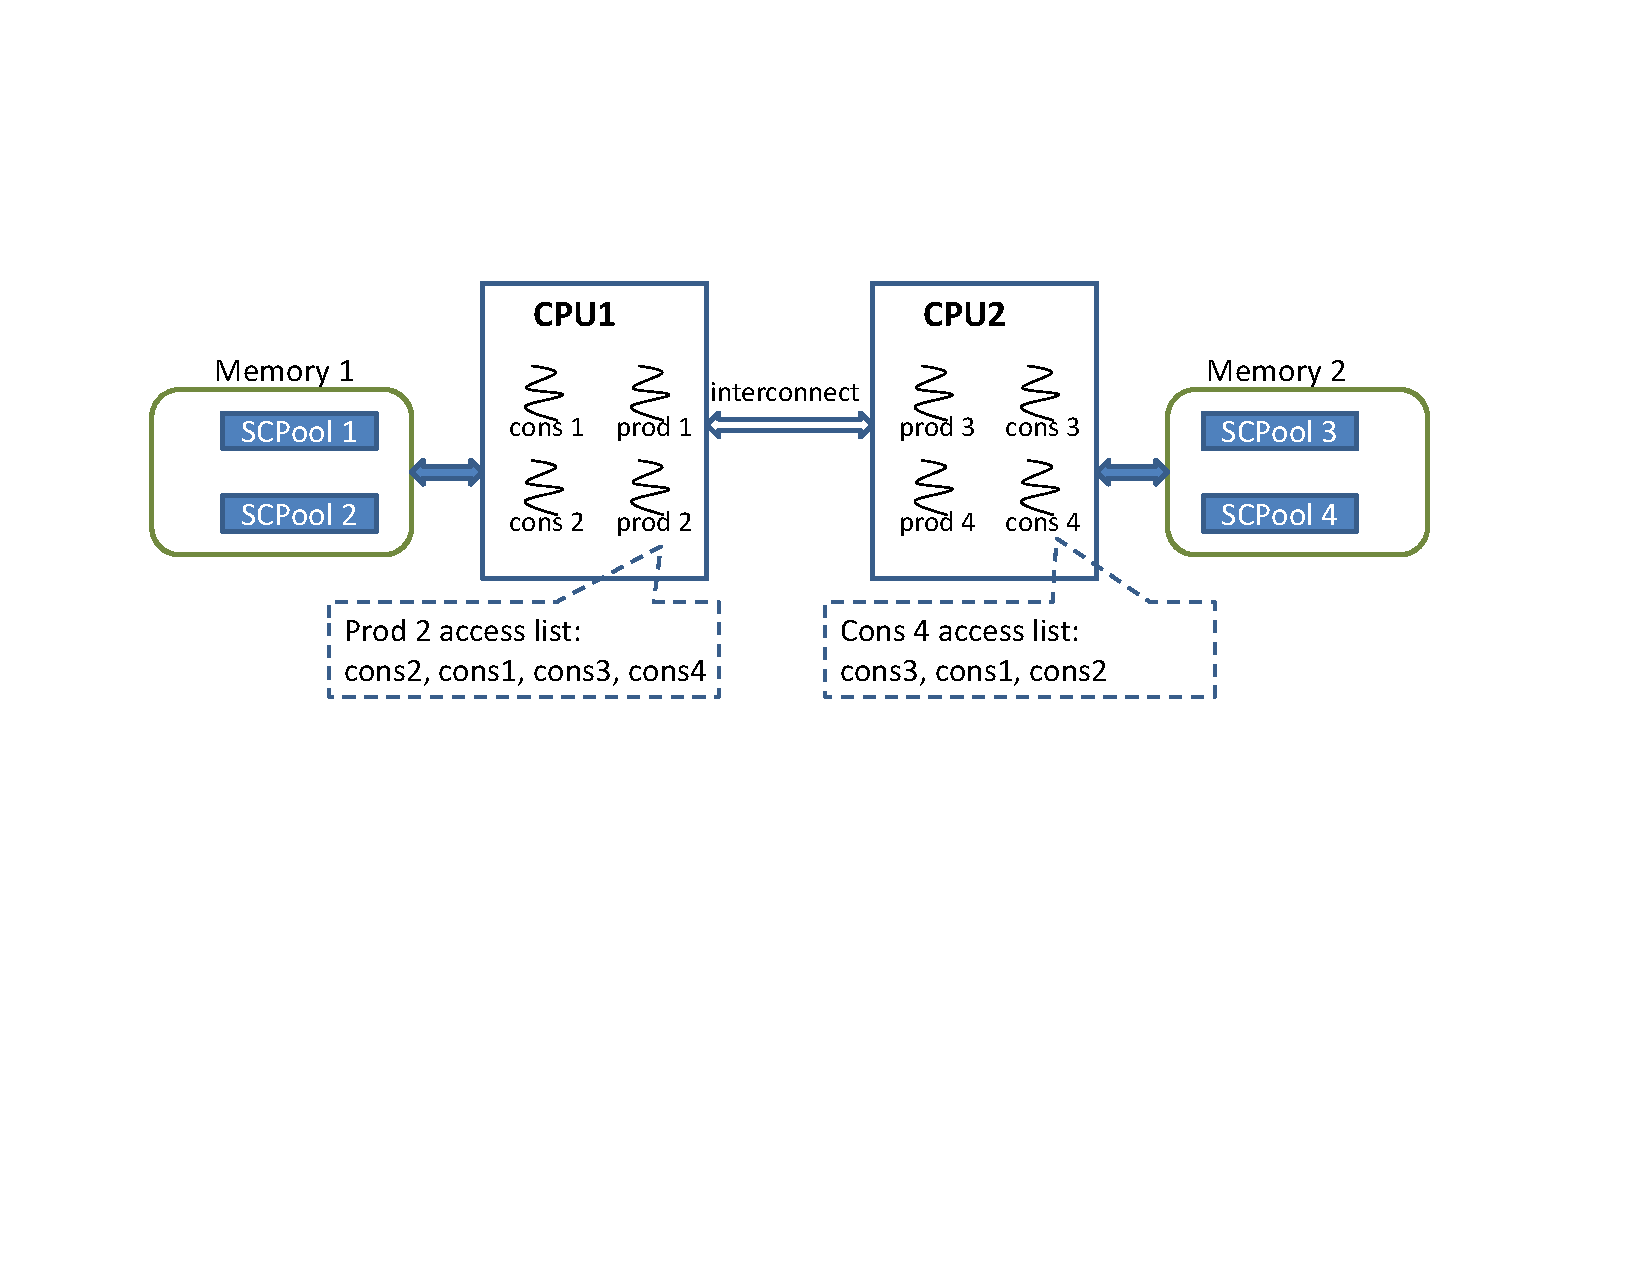
\includegraphics[width=0.7\textwidth]{figures/system-fig}
	\caption{\footnotesize{System overview of the management framework. In the given example the system is composed of two processors that are connected to their own memory banks (NUMA architecture). There are two producers and two consumers running on each processor, the data of each consumer is allocated at the closest available physical memory. A producer $p_i$ has an access list of consumers for task insertion. A consumer $c_i$ has an access list of consumers for task stealing. }}
	\label{fig:system-fig}
\end{figure}

\paragraph {Management policy.}
A management policy is generally defined by the way in which: (1) a producer chooses one of the SCPools to insert a task to, and when it chooses to use produce force; and (2) a consumer decides when to retrieve a task from its own pool and steal tasks from other pools. 
Note that the policy is independent of the underlying SCPool implementation. We believe that it is a subject for engineering optimizations, based on specific workloads and demands.


In the current work, we present a policy that exploits the locality properties of NUMA architectures and is aimed at achieving maximal throughput. If the individual SCPools themselves are lock-free and starvation-free, then our policy preserves these properties at the system level. Our policy is as follows:
\begin{itemize}
	\item {\bf Access lists.} Each process in the system (producer or consumer) is provided with an \emph{access list}, an ordered list of consumers, sorted according to their distance from that process (see Figure~\ref{fig:system-fig}). Intuitively, our policy is to have a producer mostly interact with the closest consumer, while stealing mainly happens inside the same processor node. 
	\item {\bf Producer's policy.} A producer inserting a task first calls the \emph{produce} function of the first SCPool in its access list. Note that a produce operation might fail if the pool is full, (which can be seen as evidence of that the corresponding consumer is overloaded).  In this case, the producer tries to insert the task into other pools, in the order defined by its access list. If all insertions fail, the producer invokes the \emph{produceForce} operation on the closest SCPool, which always succeeds (expanding the pool if needed). 
	\item {\bf Consumer's policy.} A consumer consumes tasks from its own SCPool. If its SCPool is empty, the consumer tries to steal tasks from other pools in the order defined by its access list. 
\end{itemize}



% The inter-pool communication policy is a subject to engineering optimizations and its optimal behavior should probably
% depend on the workload. For the purpose of our evaluation we propose the following approach. 
	% Producer policy. Each producer is provided with the list of all available consumers sorted according to the locality considerations of the given architectures. For example, in case of 
% In order to insert a task a producer first invokes a produce() operation on the closest consumer. If this operation fails, 
% then the closest consumer's pool is full (which could be evidence of an over-load of the given consumer thread) and the producer should 
% try to insert a task to another consumer. If neither consumer ... a producer finally invokes produceForce(), which expands the pool if necessary and always succeeds to insert the task. 
	% Consumer policy. A consumer works in a loop of consuming its own tasks. If the own pool of a consumer is empty, the consumer iterates over all other consumers and tries to steal tasks from there. 




\section{Algorithm Description}
\label{sec:algo}
\negspace
In the current section we present the SALSA SCPool. We first show the data structures of SALSA in Section~\ref{alg-structure}, and then present the basic algorithm without stealing support in Section~\ref{alg-overview}. The stealing procedure is described in Section~\ref{alg-stealing}, finally, the role of chunk pools is presented in Section~\ref{alg-pools}.
\negspace
\subsection{SALSA Structure\label{alg-structure}}
\newcounter{alg:non-fifo:lines}
\begin{algo}[!ht]
\caption{SALSA implementation of SCPool: Data Structures.} 
\label{alg:non-fifo-ds}
\scriptsize
\begin{minipage}[t]{0.48\textwidth}
\begin{distribalgo}[1]
\smallskip

\INDENT {{\bf Chunk type}}
	\STATE Task[CHUNK\_SIZE] tasks 
  \STATE int owner \comment {owner's consumer id}
\ENDINDENT

\INDENT {{\bf Node type}}
  \STATE Chunk c; initially $\bot$
  \STATE int idx; initially -1
  \STATE Node next; 
\ENDINDENT

\setcounter{alg:non-fifo:lines}{\value{ALC@line}} % store the line number
\end{distribalgo}
\end{minipage}%
%
\hfill
%
\begin{minipage}[t]{0.48\textwidth}
%
\begin{distribalgo}[1]
\setcounter{ALC@line}{\value{alg:non-fifo:lines}}
\smallskip

\INDENT {{\bf SALSA per consumer data structure}:}
  \STATE int consumerId
  \STATE List\tup{Node}[] chunkLists \comment {one list per producer + extra list for stealing (every list is single-writer multi-reader)} 
  \STATE Queue\tup{Chunk} chunkPool \comment {pool of spare chunks}
  \STATE Node currentNode, initially $\bot$ \comment {current node to work with} 
\ENDINDENT

\setcounter{alg:non-fifo:lines}{\value{ALC@line}}
\end{distribalgo}
\end{minipage}
\end{algo}


\begin{figure}[htb]
	\centering
	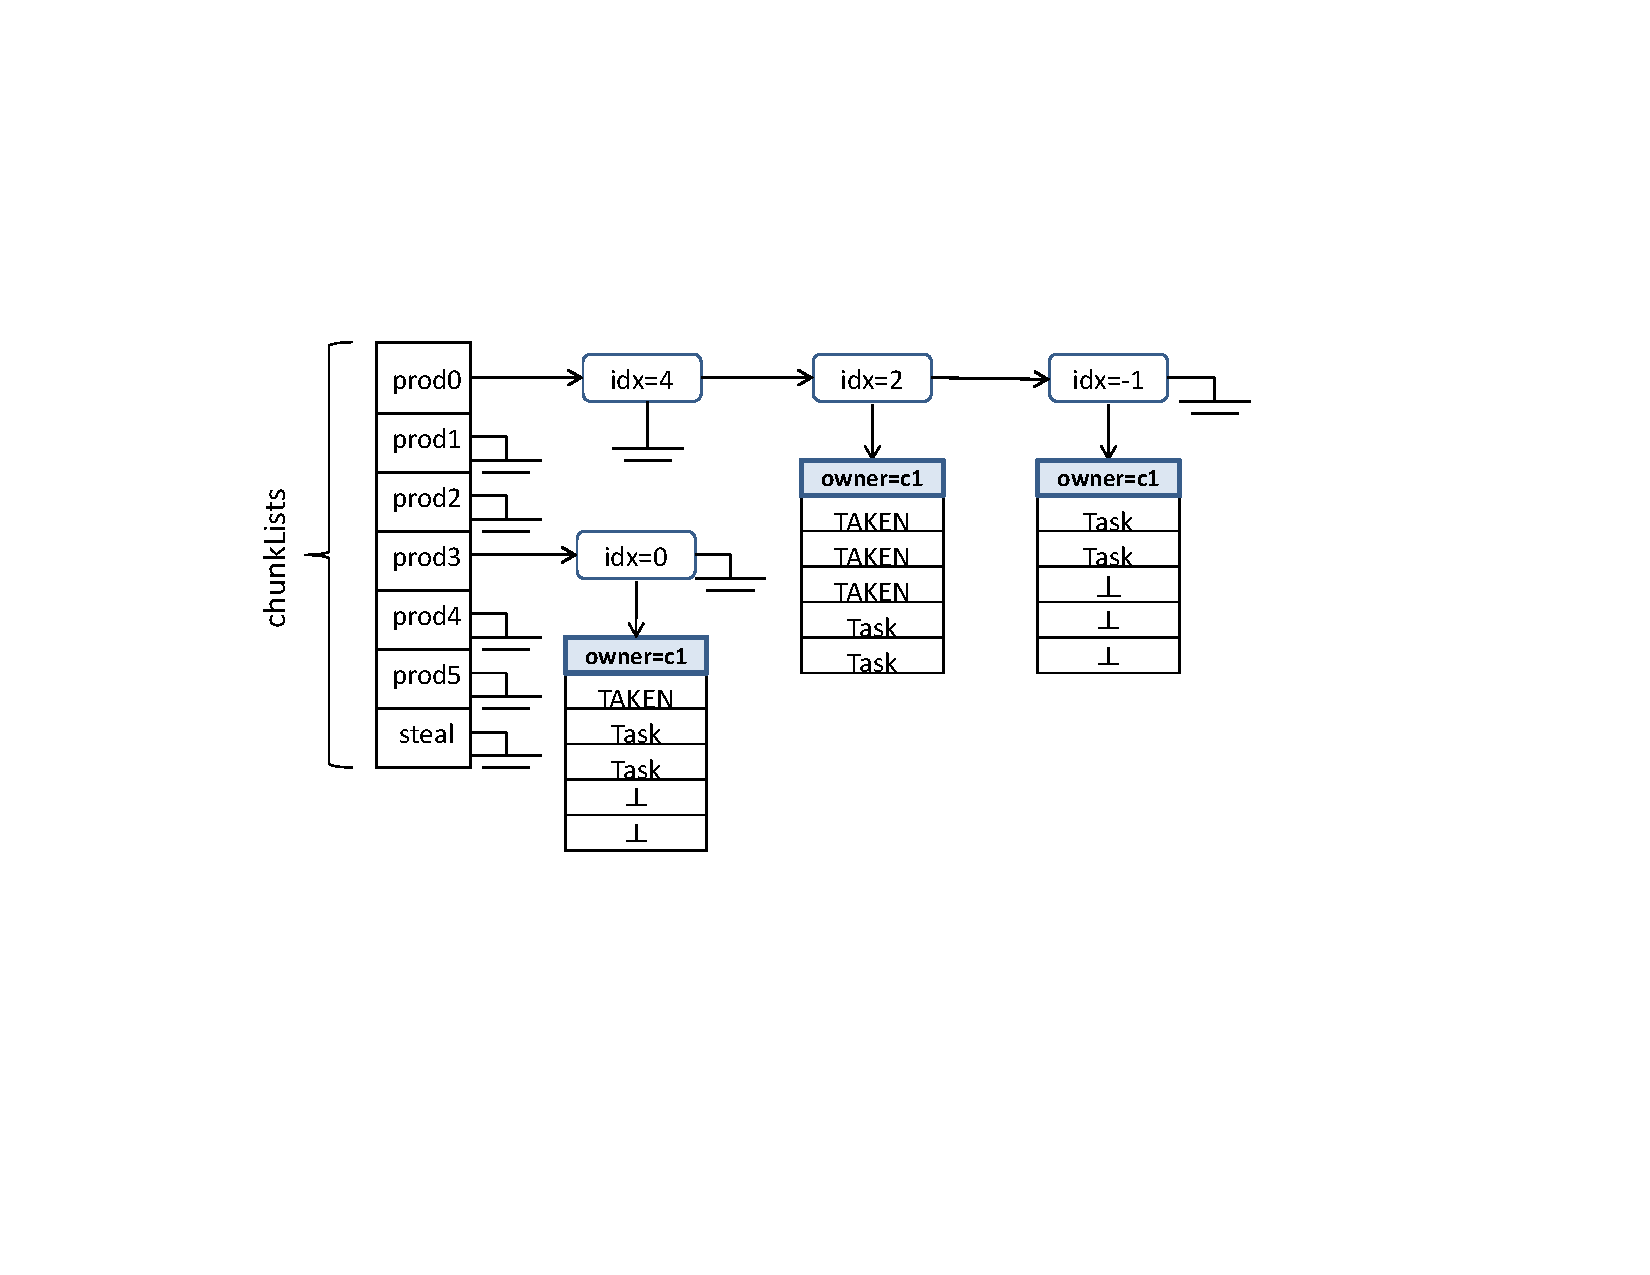
\includegraphics[height=0.3\textwidth]{figures/salsa-struct}
	\caption{
	    \footnotesize{Chunk lists in SALSA single consumer pool implementation. Tasks are kept in chunks, which are 
	    organized in per-producer lists; an additional list is reserved for stealing. Each list can be modified 
	    by the corresponding producer only. The only process that is allowed to retrieve tasks from a chunk is 
	    the owner of that chunk (defined by the ownership flag). A Node's index corresponds to the latest task taken from the chunk
	    or the task that is about to be taken by the current chunk owner. 
	    }}
	\label{fig:salsa-struct}
\end{figure}

We describe the implementation of a SALSA SCPool of some consumer $c_i$.
Its data structures are described in Algorithm~\ref{alg:non-fifo-ds} and partially depicted in Figure~\ref{fig:salsa-struct}. The tasks inserted to SALSA are kept in chunks, which are organized in per-producer chunk lists. Only the producer mapped to a given list can insert a task to any chunk in that list. Every chunk is owned by a single consumer whose id is kept in the \emph{owner} field of the chunk.
The owner is the only process that is allowed to take tasks from the chunk; if another process wants to take a task from the chunk, it should first steal the chunk and change its ownership. The owner of a chunk
residing at $c_i$'s SCPool is $c_i$ itself, unless that chunk is being stolen. A task entry in a chunk is used at most once. It holds the value $\bot$ initially, and TAKEN after the task it held has been consumed.

The per-producer chunk lists are kept in the array \emph{chunkLists} (see Figure~\ref{fig:salsa-struct}), where \emph{chunkLists[j]} keeps a list of chunks with tasks inserted by producer $p_j$. In addition, the array has a special entry \emph{chunkLists[steal]}, holding chunks stolen by $c_i$. Every list has a single writer who can modify the list structure (add or remove nodes), \emph{chunkLists[j]} can be modified only by the producer $p_j$, while the list \emph{chunkLists[steal]} can be modified only by the SCPool's owner $c_i$. Specifically, a consumed node (whose chunk was removed by the consumer) is lazily reclaimed and removed by the list's owner (typically a producer). For brevity, this is omitted from the pseudo-code bellow. Having a single writer allows us to implement the lists without synchronization primitives, similarly to the single-writer linked-list in~\cite{Michael:2004:HPS:987524.987595}.

In addition to the chunk pointer, each node keeps the index of the latest taken task. As we show in Section~\ref{alg-stealing}, this index plays a crucial role in chunk stealing. Safe memory reclamation is provided by using hazard pointers~\cite{Michael:2004:HPS:987524.987595} both for nodes and for chunks.

The free (reclaimed) chunks in SALSA are kept inside the SCPools in \emph{chunkPool}, a lock-free queue~\cite{Michael:1996:SFP:248052.248106}. These pools serve two purposes. First, they enable efficient memory reuse. Second, as we show in Section~\ref{alg-pools}, managing per-consumer chunk pools is good for load balancing. 
\negspace
\subsection{Basic Algorithm\label{alg-overview}}




The local variables and algorithms of the producer appear in
Algorithm~\ref{alg:producer-non-fifo}. The producer's code is fairly simple, the producer first
attempt to add tasks to the chunks it previously used, if this is the first produce action or the
previous chunk was already filled, the producer will attempt to take a chunk from the chunk pool and
add it to its list on the pool of the given consumer. If the pool is empty the operation will fail
with a FULL message, if produceForce was called the operation will not fail, instead a new chunk
will be allocated. 


\negspace
\subsection{Stealing\label{alg-stealing}}
The stealing algorithm is presented in a function {\bf steal()} in Algorithm~\ref{alg:non-fifo}. 
We refer to the stealing consumer as $c_s$, the victim process whose chunk is being stolen is called $c_v$, and the stolen chunk is referred to as $ch$.

The idea is to turn $c_s$ to the exclusive consumer of $ch$, such that $s_c$ will be able to take tasks from the chunk without synchronization. 
In order to do that, $c_s$ changes the ownership of $ch$ (line~\ref{alg:line:chown}) and removes the chunk from the list of $c_v$ (line~\ref{alg:line:remove-chunk}). 
Once $c_v$ notices the change in the ownership it stops taking tasks from $ch$ (lines~\ref{alg:lines:stolen-chunk-end}--\ref{alg:lines:stolen-chunk-begin}). 

When the {\bf steal()} operation of $c_s$ occurs simultaneously with the {\bf takeTask()} operation of $c_v$, both $c_s$ and $c_v$ might try to retrieve the same task. Hence, $c_v$ notifies potential stealers of the task it is about to take by incrementing the \emph{idx} value of the $ch$'s node (line~\ref{alg:lines:ind-inc}). This value is later read by $c_s$ in line~\ref{alg:line:copy-prev-node} when creating a copy of $ch$'s node.

%Consider, for example, a scenario in which the $idx$ value is incremented from $10$ to $11$ during $c_v$'s {\bf takeTask()} operation.
Consider, for example, a scenario in which the $idx$ is incremented by $c_v$ from $10$ to $11$. 
If $c_v$ checks the ownership before it is changed by $c_s$, then $c_v$ takes the task at $11$ without synchronization (see line~\ref{alg:lines:fast-path}). Therefore, $c_s$ is never allowed to take a task pointed by \emph{idx}, and hence $c_v$ has to take the task at $11$ even if it observes the ownership change. 
After taking the chunk, $c_s$ will eventually try to take a task pointed by $idx+1$. However, if $c_s$ read $idx$ before it was incremented by $c_v$, $c_s$ might think that the value of $idx+1$ is $11$. In this case, both $c_s$ and $c_v$ will try to retrieve the task at $11$, hence both should use CAS operation in order to retrieve a task: line~\ref{alg:line:cas-steal} for $c_s$ and line~\ref{alg:line:cas-consumer} for $c_v$. 

The above algorithm works correctly as long as the stealing consumer can observe the node with the updated index value. 
This might not be a case if the same chunk is concurrently stolen by another consumer because the \emph{idx} of the original node would be obsolete. 
In order to prevent this situation, stealing a chunk from the pool of consumer $c_v$ is allowed only if $c_v$ is the owner of this chunk (line~\ref{alg:line:chown}). 

A naive way for $c_s$ to steal the chunk from $c_v$ would be first to change the ownership and then to move the chunk to the steal list. However, that would make our algorithm blocking because there exists a time that the chunk is unaccessible via the lists of $c_s$ and yet $c_s$ is its owner. In this case, as we explained above, the chunk cannot be stolen, which prevents taking the tasks from this chunk by other consumers. Therefore, our solution is to first add the original node to the steal list of $c_s$, change the ownership, and only then to replace the original node with a new node (lines~\ref{alg:line:resteal-begin}--\ref{alg:line:resteal-end}). 
 

% change the ownership (the consumer will check the ownership change)
% what about the first task retrieval? (the description includes the explanation about idx+1)
% what about concurrent stealing? (I want to see the updated idx value, the updated idx value is kept at node, hence I need to steal from the owner only)
% what about non-blocking properties? (want to allow others to always find a task...) 






% \paragraph{Stealing the chunk.} Before stealing a chunk, $c_1$ has to make sure $c_2$ will not take any more tasks from that chunk, so the $c_1$ may later take tasks with no need for synchronization. To achieve this $c_1$ must change the owner field of the chunk. Changing the ownership will prevent $c_2$ from taking tasks as a consumer always checks that he is the owner of the chunk before taking tasks. 
% 
% Before changing the ownership we must relate to two issues: (1) Stealing a chunk from the pool of consumer $c_2$ is allowed only if $c_2$ is the owner of the chunk that we steal, this is needed so it is guaranteed that $c_2$ reads the latest value of the idx, which is only found in the owner's node. (2) We want that other consumers would be able to steal the chunk during the process, so that the algorithm will stay lock-free. 
% 
% For those two reasons we must make the chunk accessible via $c_1$'s pool before changing ownership. However, we cannot simply add a new node to $c_1$'s steal list, as that node's idx field will not be updated if $c_2$ changes his idx field. Therefore, before changing ownership, $c_1$ adds $c_2$'s node to his steal list (Line~\ref{} in Algorithm~\ref{}). Now $c_1$ takes ownership (Line~\ref{}) and creates a new node with the updated idx that will replace the $c_2$'s node (Line~\ref{}), as the original idx may only change by one pending operation at most. Finally $c_1$ changes $c_2$'s node to point to NULL (Line~\ref{}) so that this node will not be used and will be lazily removed.
% 
% \paragraph{Taking the first task.} After the $c_1$ stole the chunk, he must attempt to take a task, so Property~\ref{steal-progress-property} will hold. $c_1$ will try to take the task at $idx+1$, however, this task may be also taken by $c_2$ if he started a consume operation before $c_1$ completed the node transfer. This is why $c_1$ must use a CAS operation to take this node (Line~\ref{}). $c_2$ must also attempt to take this node (Line~\ref{}) even if he noticed the ownership change, since he does not know if $c_1$ read the idx value before or after $c_2$ increased it Line~\ref{}.

% \vspace{5mm}\noindent
% We claim that the steal operation hold Property~\ref{steal-progress-property}. In line~\ref{} a chunk with at least one task is taken, therefore there is a task at $idx+1$. if $idx$ is updated during the stealing operation it means that the original consumer is taking that task and therefore the property holds. Otherwise, either the CAS in line~\ref{} failed and another consumer successfully stole the chunk and will return a task, or the current producer will reach line~\ref{}. In this line the CAS will be executed if the task wasn't already taken, and since either the stealing consumer or the original consumer will succeed performing the CAS.
\negspace
\subsection{Chunk Pools\label{alg-pools}}
As described in Section~\ref{alg-structure}, each consumer keeps a pool of free chunks.
When a producer needs a new chunk for adding a task to consumer $c_i$, it tries to get a chunk from $c_i$'s chunk pool -- if no free chunks are available, the {\bf produce()} operation fails.

As described in Section~\ref{sec:system}, our system-wide policy defines that if an insertion operation fails, then the producer tries to insert a task to other pools. Thus, the producer avoids adding tasks to overloaded consumers, which in turn decreases the amount of costly steal operations. 

Another SALSA property is that a chunk is returned to the pool of a consumer that retrieves the latest task of this chunk. 
Therefore, the size of the chunk pool of consumer $c_i$ is proportional to the rate of $c_i$'s task consumption.
This property is especially appealing for heterogeneous systems -- a faster consumer $c_i$ ", (e.g., one running on a stronger or less loaded core), will have a larger chunk pool, and so more {\bf produce()} operations will insert tasks to $c_i$, automatically balancing the overall system load. 

\newcounter{alg:non-fifo:lines}
\begin{algo}[!ht]
\caption{Non-FIFO implementation of SCPool: Data Structures.} 
\label{alg:non-fifo-ds}
\scriptsize
\begin{minipage}[t]{0.48\textwidth}
\begin{distribalgo}[1]
\smallskip

\INDENT {{\bf Chunk data structure}:}
	\STATE Task[CHUNK\_SIZE] tasks 
  \STATE int owner \comment {owner's consumer id}
\ENDINDENT

\INDENT {{\bf Node data structure}:}
  \STATE Chunk c; initially $\bot$
  \STATE int idx; initially -1
\ENDINDENT

\setcounter{alg:non-fifo:lines}{\value{ALC@line}} % store the line number
\end{distribalgo}
\end{minipage}%
%
\hfill
%
\begin{minipage}[t]{0.48\textwidth}
%
\begin{distribalgo}[1]
\setcounter{ALC@line}{\value{alg:non-fifo:lines}}
\smallskip

\INDENT {{\bf SCPool per consumer data structure}:}
  \STATE int consumerId
  \STATE List\tup{Node}[] chunkLists \comment {one list per producer + extra list for stealing (single-writer multi-reader)} 
  \STATE ChunkPool chunkPool \comment {the pool of spare chunks}
  \STATE Node currentNode, initially $\bot$ \comment {current node to work with} 
\ENDINDENT

\setcounter{alg:non-fifo:lines}{\value{ALC@line}}
\end{distribalgo}
\end{minipage}
\end{algo}

\begin{algo}[!ht]
\caption{Non-FIFO implementation of SCPool: Producer Functions.}
\label{alg:producer-non-fifo}
\scriptsize
\begin{minipage}[t]{0.48\textwidth}
\begin{distribalgo}[1]
\setcounter{ALC@line}{\value{alg:non-fifo:lines}}

\INDENT {{\bf Producer local variables}:}
	\STATE int producerId
	\STATE Chunk chunk; initially $\bot$ \comment {the chunk to insert to}
	\STATE int prodIdx; initially $0$ \comment {the prefix of inserted tasks}
\ENDINDENT

\setcounter{alg:non-fifo:lines}{\value{ALC@line}} % store the line number
\end{distribalgo}
\end{minipage}%
%
\hfill
%
\begin{minipage}[t]{0.48\textwidth}
%
\begin{distribalgo}[1]
\setcounter{ALC@line}{\value{alg:non-fifo:lines}}

\INDENT {{\bf Function produce}(Task t, SCPool scPool):}
	\INDENT {{\bf if} (chunk $= \bot$) {\bf then}}
		\STATE newChunk $\leftarrow$ a chunk from scPool.chunkPool
		\STATE {\bf if} (chunk $= \bot$) {\bf then return FULL} \comment {no available chunks}
		\STATE newChunk.owner $\leftarrow$ scPool.consumerId
		\STATE node $\leftarrow$ new node with idx $=-1$ and c $=$ newChunk
		
		\STATE scPool.chunkLists[producerId].{\bf append}(node)
		\STATE chunk $\leftarrow$ newChunk; prodIdx $\leftarrow 0$ 
	\ENDINDENT
	\STATE chunk.tasks[prodIdx] $\leftarrow$ t; prodIdx++
	\INDENT {{\bf if}(prodIdx $=$ CHUNK\_SIZE) {\bf then}}
	  \STATE chunk $\leftarrow \bot$ \comment {the chunk is full}
	\ENDINDENT
	\STATE {\bf return SUCCESS}
\ENDINDENT

\setcounter{alg:non-fifo:lines}{\value{ALC@line}}
\end{distribalgo}
\end{minipage}
\end{algo}

\begin{algo}[!ht]
\caption{Non-FIFO implementation of SCPool: Consumer Functions.} 
\label{alg:non-fifo}
\scriptsize
\begin{minipage}[t]{0.48\textwidth}
\begin{distribalgo}[1]
\setcounter{ALC@line}{\value{alg:non-fifo:lines}}
\smallskip


\INDENT {{\bf Function consume}():}
  \INDENT {{\bf if}(currentNode $\neq \bot$) {\bf then} \comment {common case}}
		\STATE t $\leftarrow$ {\bf takeTask}(currentNode)
		\STATE {\bf if} (t $\neq \bot$) {\bf then return} t
	\ENDINDENT
	\comment {Iterate over other chunk lists}
	\INDENT {{\bf foreach} cl {\bf in} chunkLists {\bf do} \comment {fair traversal}} 
  	\INDENT {{\bf foreach} node {\bf in} cl {\bf do}}
  		\STATE t $\leftarrow$ {\bf takeTask}(node)
			\STATE {\bf if} (t $\neq \bot$) {\bf then} currentNode $\leftarrow$ node; {\bf return} t
  	\ENDINDENT
	\ENDINDENT
	\STATE currentNode $\leftarrow \bot$; {\bf return} $\bot$
\ENDINDENT

\medskip

\INDENT {{\bf Function takeTask}(Node n):}
  \STATE chunk $\leftarrow$ n.c
  \STATE {{\bf if} (chunk $= \bot$) {\bf then return $\bot$} \comment{this chunk has been stolen}}
 
  \STATE task $\leftarrow$ chunk.tasks[n.idx + 1]
  \STATE {\bf if} (task $= \bot$) {\bf then return} $\bot$ \comment{no inserted tasks}
 	
 	\smallskip 
  \STATE n.idx++ \comment {tell the world you're going to take a task from idx}
  \INDENT {{\bf if} (chunk.owner $=$ consumerId) {\bf then} \comment {common case}}
 		\STATE chunk.tasks[n.idx] $\leftarrow$ TAKEN
  	\INDENT {{\bf if}(n.idx + 1 $=$ CHUNK\_SIZE) {\bf then} \comment {finished the chunk}}
  		\STATE n.c $\leftarrow \bot$; return the chunk to the chunkPool
  		\STATE currentNode $\leftarrow \bot$
  	\ENDINDENT
  	\STATE {\bf return} task 
  \ENDINDENT
  
  \smallskip
  \comment {the chunk has been stolen, CAS the last task and go away}
 	\STATE success $\leftarrow$ (task $\neq$ TAKEN $\wedge$ \\
 		\hspace{0.5cm} CAS(chunk.tasks[n.idx], task, TAKEN))
	\STATE n.c $\leftarrow \bot$; currentNode $\leftarrow \bot$
 	\STATE {\bf return} (success) ? task : $\bot$
\ENDINDENT

\setcounter{alg:non-fifo:lines}{\value{ALC@line}} % store the line number
\end{distribalgo}
\end{minipage}%
%
\hfill
%
\begin{minipage}[t]{0.48\textwidth}
%
\begin{distribalgo}[1]
\setcounter{ALC@line}{\value{alg:non-fifo:lines}}
\smallskip

\INDENT {{\bf Function steal}(SCPool from):}
	\STATE prevNode $\leftarrow$ a node holding tasks from some list \comment {different policies possible}
	\STATE c $\leftarrow$ prevNode.c;
  \STATE {\bf if} (c = $\bot$) {\bf then return} $\bot$

	\comment {add prevNode to steal list to make it re-stealable}
  \STATE chunkLists[steal].{\bf append}(prevNode)
  \INDENT {{\bf if} ({\bf CAS}(c.owner, from.consumerId, consumerId) $=$ false)}
 		\STATE chunkLists[steal].{\bf remove}(prevNode)
 		\STATE {\bf return} $\bot$ \comment {failed to steal}
	\ENDINDENT
	\STATE {\bf if}(prevNode.idx $+1$) {\bf then}
	\smallskip
	\STATE newNode $\leftarrow$ copy of prevNode
	\STATE replace prevNode with newNode in chunkLists[steal]
	\STATE prevNode.c $\leftarrow \bot$ \comment {done stealing the chunk, take its task}
	
	\smallskip
	\STATE idx $\leftarrow$ newNode.idx
	\STATE task $\leftarrow$ c.tasks[idx+1] 
	\STATE {\bf if} (task $= \bot$) {\bf then return} $\bot$ \comment {still no task at idx+1}
	\INDENT {{\bf if} (task $=$ TAKEN $\vee$ \\
		\hspace{0.5cm} !CAS(c.tasks[idx+1], task, TAKEN)) {\bf then}} 
		\STATE task $\leftarrow \bot$
	\ENDINDENT
	\STATE currentNode $\leftarrow$ newNode
	\INDENT {{\bf if}(newNode.idx + 1 $=$ CHUNK\_SIZE) {\bf then}}
  	\STATE newNode.c $\leftarrow \bot$; return the chunk to the chunkPool
  	\STATE currentNode $\leftarrow \bot$
  \ENDINDENT
	\STATE newNode.idx $\leftarrow$ newNode.idx+1
	\STATE {\bf return} task
\ENDINDENT

\setcounter{alg:non-fifo:lines}{\value{ALC@line}}
\end{distribalgo}
\end{minipage}
\end{algo}

%\begin{algo}[!ht]
%\caption{Non-FIFO implementation of SCPool: Auxiliary Functions.} 
%\label{alg:non-fifo-aux}
%\scriptsize
%\begin{minipage}[t]{0.48\textwidth}
%\begin{distribalgo}[1]
%\setcounter{ALC@line}{\value{alg:non-fifo:lines}}
%\smallskip
%
%\INDENT {{\bf Function getStealingScore}():}
%	\comment {return the max of all the chunkCounters}
%	\STATE res $\leftarrow 0$
%	\INDENT {{\bf for} i $= 0, \ldots, $ NUM\_PRODUCERS {\bf do}}
%		\STATE {\bf if} (chunkCounters[i] $>$ res) res $\leftarrow$ chunkCounters[i]
%	\ENDINDENT
%	\STATE {\bf return} res
%\ENDINDENT
%
%\medskip
%\INDENT {{\bf Function isEmpty}(Node n):}
%  \STATE c $\leftarrow$ n.chunk
%  \STATE {\bf if} (c $= \bot$) {\bf then return true}
%  \STATE \comment {in empty chunk $\bot_2$ values are followed by $\bot$ values}
%  \INDENT {{\bf for} i $=$ n.idx, $\ldots$, i $<$ CHUNK\_SIZE {\bf do}}
%    \STATE {\bf if} (c.tasks[i] $= \bot$) {\bf then return true}
%    \STATE {\bf if} (c.tasks[i] $\neq \bot_2$) {\bf then return false} \comment {a task found}
%  \ENDINDENT
%  \STATE {\bf return true} \comment {no tasks found}
%\ENDINDENT
%
%\setcounter{alg:non-fifo:lines}{\value{ALC@line}} % store the line number
%\end{distribalgo}
%\end{minipage}%
%%
%\hfill
%%
%\begin{minipage}[t]{0.48\textwidth}
%%
%\begin{distribalgo}[1]
%\setcounter{ALC@line}{\value{alg:non-fifo:lines}}
%\smallskip
%\INDENT {{\bf Function chooseEntryForSteal}(SCPool from):}
%	\STATE maxNumChunks $\leftarrow 0$
%	\INDENT {{\bf for} i $= 0, \ldots, $ NUM\_PRODUCERS {\bf do}}
%		\INDENT {{\bf if} (from.chunkCounters[i] $>$ maxNumChunks) {\bf then}}
%			\STATE maxNumChunks $\leftarrow$ from.chunkCounters[i]
%			\STATE entryForSteal $\leftarrow$ i
%		\ENDINDENT
%	\ENDINDENT
%	\STATE {\bf return} entryForSteal
%\ENDINDENT
%
%\medskip
%
%\INDENT {{\bf Function removeNode}(Node n):}
%	\STATE {\bf FetchAndAdd}(chunkCounters[currentEntry],-1)
%	\STATE prodEntries[currentEntry].{\bf remove}(n)
%	\STATE currentNode $\leftarrow \bot$
%\ENDINDENT 
%
%\medskip
%
%\INDENT {{\bf Function checkLast}(Node n, Chunk c):}
%	\STATE {\bf if}(n.idx $+1 \neq $ CHUNK\_SIZE) {\bf then return}
%	\STATE \comment {this thread took the last task --- reclaiming}
%  \STATE {\bf reclaimChunk}(c); {\bf removeNode}(n)
%\ENDINDENT
%
%\setcounter{alg:non-fifo:lines}{\value{ALC@line}}
%\end{distribalgo}
%\end{minipage}
%\end{algo}


\section{Evaluation}
\label{sec:evaluation}

\section{Conclusions}
\label{sec:conclusions}

\bibliographystyle{abbrv}
\bibliography{refs}

\end{document}